%\documentclass[hyperref={pdfpagelabels=false}]{beamer}
\documentclass{beamer}
\usepackage{textcomp}
\usepackage[german]{babel}
\usepackage[utf8]{inputenc}
\usepackage{times}
\usepackage[T1]{fontenc}
\usepackage{bytefield}

%gets rid of navigation symbols
\setbeamertemplate{navigation symbols}{}

\mode<presentation>
{
  \usetheme{Marburg}
  \setbeamercovered{transparent}
}

\title {Networked Embedded Systems VU}
\subtitle {Clock Synchronisation\\over a\\ leightweight protocol with basic fault tolerance}
\author{R. Annessi,\\ A. Heinisch,\\ N. Mayerhofer}

% custom date
\usepackage{datetime}
\newdateformat{customdate}{\monthname{ }\THEYEAR}
\date{\customdate\today}


\logo{

\includegraphics[height=0.5cm]{./images/logo_neu.jpg}
}


\begin{document}
\begin{frame}
  \titlepage
\end{frame}
% logo only on title page
 \logo{}

\begin{frame}{Structure of presentation}
  \tableofcontents
\end{frame}


\section{Project Outline}
\begin{frame}{Motivation}
\begin{center}
\begin{itemize}
  \item Embedded communication for home automation are expensive
    \begin{itemize}
      \item Certification necessary
      \item Licence needed
      \item ...
    \end{itemize}
  \item Implementation of existing protocols are often resource intensive
  \item Migration of additional components in given systems needs expertise
\end{itemize}
\end{center}
\end{frame}

\begin{frame}{Project goals}
\begin{center}
\begin{itemize}
 \item \begin{large}Masterless\end{large}
 \item \begin{large}Up to 450m bus length\end{large}
 \item \begin{large}Usable for small microcontrollers\end{large}
 \item \begin{large}Low configuration overhead\end{large}
 \item \begin{large}Provide basic fault tolerance\end{large}
 \item \begin{large}Easily adaptable to existing projects\end{large}
 \item \begin{large}Easily migrateable from existing systems\end{large}
 \item \begin{large}Separation of communication and application layers\end{large}
\end{itemize}
\end{center}

\end{frame}

\section{Group subject}
\begin{frame}{Group subject}{Clock synchronisation}
  \begin{itemize}
    \item \begin{large}Comparison of clock synchronisation algorithms\end{large}
    \item \begin{large}Implementation of an algorithm including\end{large}
      \begin{itemize}
	\item Time estimation
	\item Feasibility estimation
      \end{itemize}
    \item \begin{large}Testing under fault conditions\end{large}
  \end{itemize}
\end{frame}


\section{Bus Protocol}
\begin{frame}{Bus protocol}{Layer 1}
\begin{center}
\begin{itemize}
 \item \begin{large}One wire\end{large}
 \item \begin{large}USART 9N1 configuration\end{large}
\end{itemize}
\vspace{1cm}
\begin{bytefield}{11}
 \bitheader{0-1,9-10}\\
 \bitbox{1}{S} \bitbox{9}{Datenbits} \bitbox{1}{S}\\
\end{bytefield}
\end{center}
\end{frame}


\begin{frame}{Bus protocol}{Layer 2}
\begin{center}
\begin{itemize}
  \item \begin{large}Bus tailored to our needs\end{large}
  \item \begin{large}Bus arbitration\end{large}
  \item \begin{large}CSMA/CA\end{large}
  \item \begin{large}Non-starvation handling\end{large}
  \item \begin{large}Re/integration handling\end{large}
\end{itemize}
\end{center}
\end{frame}


\begin{frame}{Bus protocol}{Layer 2: message format}
\begin{center}
   \begin{bytefield}{24}
     \bitheader{0,3-4,9-10,15-16,23}\\
     \bitbox{4}{Type} \bitbox{6}{Dest ID} \bitbox{6}{Src ID} \bitbox{8}{Len}\\
     \bitbox[lrt]{8}{Data<0>} \bitbox[lrt]{8}{Data<1>} \bitbox[lrt]{8}{..}\\ 
     \skippedwords \\
     \bitbox[lrb]{8}{..}\bitbox[lrb]{8}{Data<Len-2>}\bitbox[lrb]{8}{Data<Len-1>}\\
     \bitbox[lrb]{8}{CRC<0>}\bitbox{8}{..}\bitbox{8}{CRC<3>}\\
   \end{bytefield}
\end{center}
\end{frame}


\begin{frame}{Bus protocol}{Basic fault tolerance \& non starvation handling}
\begin{center}
\begin{itemize}
 \item \begin{large}Timer / watchdog\end{large}
\end{itemize}
\begin{center}
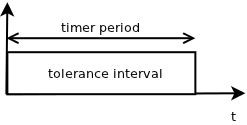
\includegraphics[width=0.7\textwidth]{./images/faulttolerance.png}
\end{center}
\end{center}
\end{frame}

%welche gibts?
%vergleichen
%welche kommen in Frage
\section{Clock Synchronisation}
\begin{frame}{Clock Synchronisation}{Variations \& pitfalls}
\begin{center}
\begin{itemize}
  \item \begin{large}Assumption of timebase\end{large}
  \item \begin{large}Clock synchronisation vs. message ordering\end{large}
  \item \begin{large}Adjustment method\end{large}
  \item \begin{large}Latency correction\end{large}
\end{itemize}
\end{center}
\end{frame}


\begin{frame}{Clock Synchronisation}{Clocks \& methods}
  \begin{center}
  \begin{itemize}
    \item \begin{large}Clock type\end{large}
    \begin{itemize}
      \item Centralized
      \item Distributed
    \end{itemize}
    \item \begin{large}Distributed clock algorithms\end{large}
    \begin{itemize}
      \item Precision time protocol
      \item Reference broadcast synchronisation
    \end{itemize}
  \item \begin{large}Method we use\end{large}
  \end{itemize}
  \end{center}
\end{frame}


\section{Time Plan}
\begin{frame}{Time Plan}
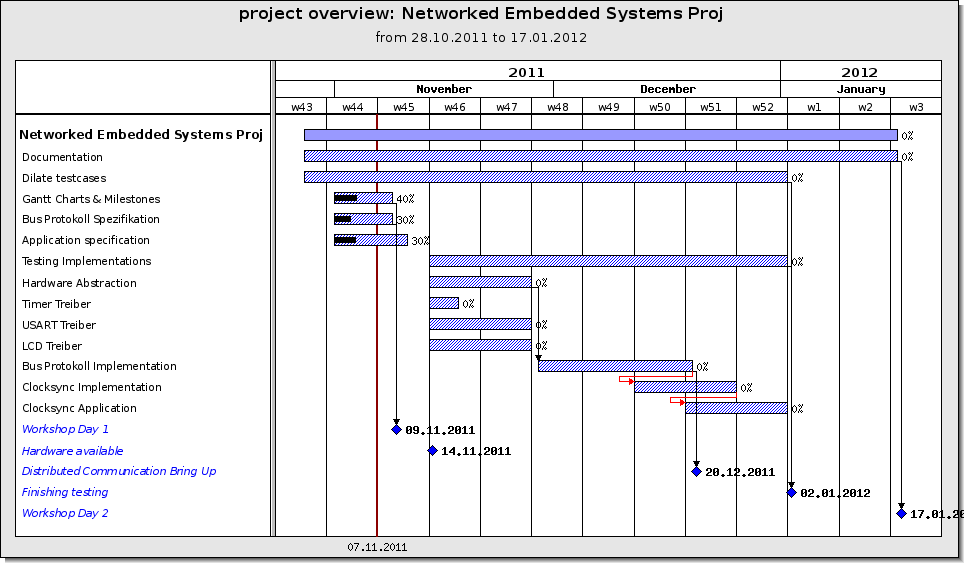
\includegraphics[width=1.0\textwidth]{./images/201111_ganttchart.png}
\vspace{1cm}
\end{frame}

\begin{frame}
\begin{center}
\begin{Huge}\textbf{Thank you!}\end{Huge}
\end{center}
\end{frame}


\begin{frame}{Questions}
\begin{center}

\includegraphics[width=0.7\textwidth]{./images/question-marks.png}
\end{center}
\end{frame}


\end{document}
